\documentclass[a4paper, fleqn]{article}
\usepackage[utf8]{inputenc}
\usepackage{amsmath}
\usepackage{amssymb}
\usepackage{caption}
\usepackage{mathtools}
\usepackage{amsfonts}
\usepackage{lastpage}
\usepackage{tikz}
\usepackage{float}
\usepackage{textcomp}
\usetikzlibrary{patterns}
\usepackage{pdfpages}
\usepackage{gauss}
\usepackage{fancyvrb}
\usepackage[table]{colortbl}
\usepackage{fancyhdr}
\usepackage{graphicx}
\usepackage{pdfpages}
\usepackage[margin=2.5 cm]{geometry}

% algorithms
\usepackage{algorithm}      % algorithm float environment
\usepackage[noend]{algpseudocode}  % from algorithmicx; no "end" on functions
\newcommand*\Let[2]{\State #1 $\gets$ #2}
\algnewcommand{\LineComment}[1]{\State \(\sslash\) #1}
\algrenewcommand\algorithmiccomment[1]{\hfill\(\sslash\) #1}
\algrenewcommand\algorithmicrequire{\textbf{Precondition:}}

\setlength\parindent{0pt}
\setlength\mathindent{75pt}

\definecolor{listinggray}{gray}{0.9}
\usepackage{listings}
\lstset{
	language=,
	literate=
		{æ}{{\ae}}1
		{ø}{{\o}}1
		{å}{{\aa}}1
		{Æ}{{\AE}}1
		{Ø}{{\O}}1
		{Å}{{\AA}}1,
	backgroundcolor=\color{listinggray},
	tabsize=3,
	rulecolor=,
	basicstyle=\scriptsize,
	upquote=true,
	aboveskip={0.2\baselineskip},
	columns=fixed,
	showstringspaces=false,
	extendedchars=true,
	breaklines=true,
	prebreak =\raisebox{0ex}[0ex][0ex]{\ensuremath{\hookleftarrow}},
	frame=single,
	showtabs=false,
	showspaces=false,
	showlines=true,
	showstringspaces=false,
	identifierstyle=\ttfamily,
	keywordstyle=\color[rgb]{0,0,1},
	commentstyle=\color[rgb]{0.133,0.545,0.133},
	stringstyle=\color[rgb]{0.627,0.126,0.941},
  moredelim=**[is][\color{blue}]{@}{@},
}

\lstdefinestyle{base}{
  emptylines=1,
  breaklines=true,
  basicstyle=\ttfamily\color{black},
}

\pagestyle{fancy}
\def\checkmark{\tikz\fill[scale=0.4](0,.35) -- (.25,0) -- (1,.7) -- (.25,.15) -- cycle;}
\newcommand*\circled[1]{\tikz[baseline=(char.base)]{
            \node[shape=circle,draw,inner sep=2pt] (char) {#1};}}
\newcommand*\squared[1]{%
  \tikz[baseline=(R.base)]\node[draw,rectangle,inner sep=0.5pt](R) {#1};\!}
\newcommand{\comment}[1]{%
  \text{\phantom{(#1)}} \tag{#1}}
\def\el{[\![}
\def\er{]\!]}
\def\dpip{|\!|}
\def\MeanN{\frac{1}{N}\sum^N_{n=1}}
\cfoot{Page \thepage\ of \pageref{LastPage}}
\DeclareGraphicsExtensions{.pdf,.png,.jpg}
\author{Nikolaj Dybdahl Rathcke (Student ID: 74763954)}
\title{Cryptography and Coding Theory \\ Assignment 2}
\lhead{Cryptography and Coding Theory}
\rhead{Assignment 2}

\begin{document}

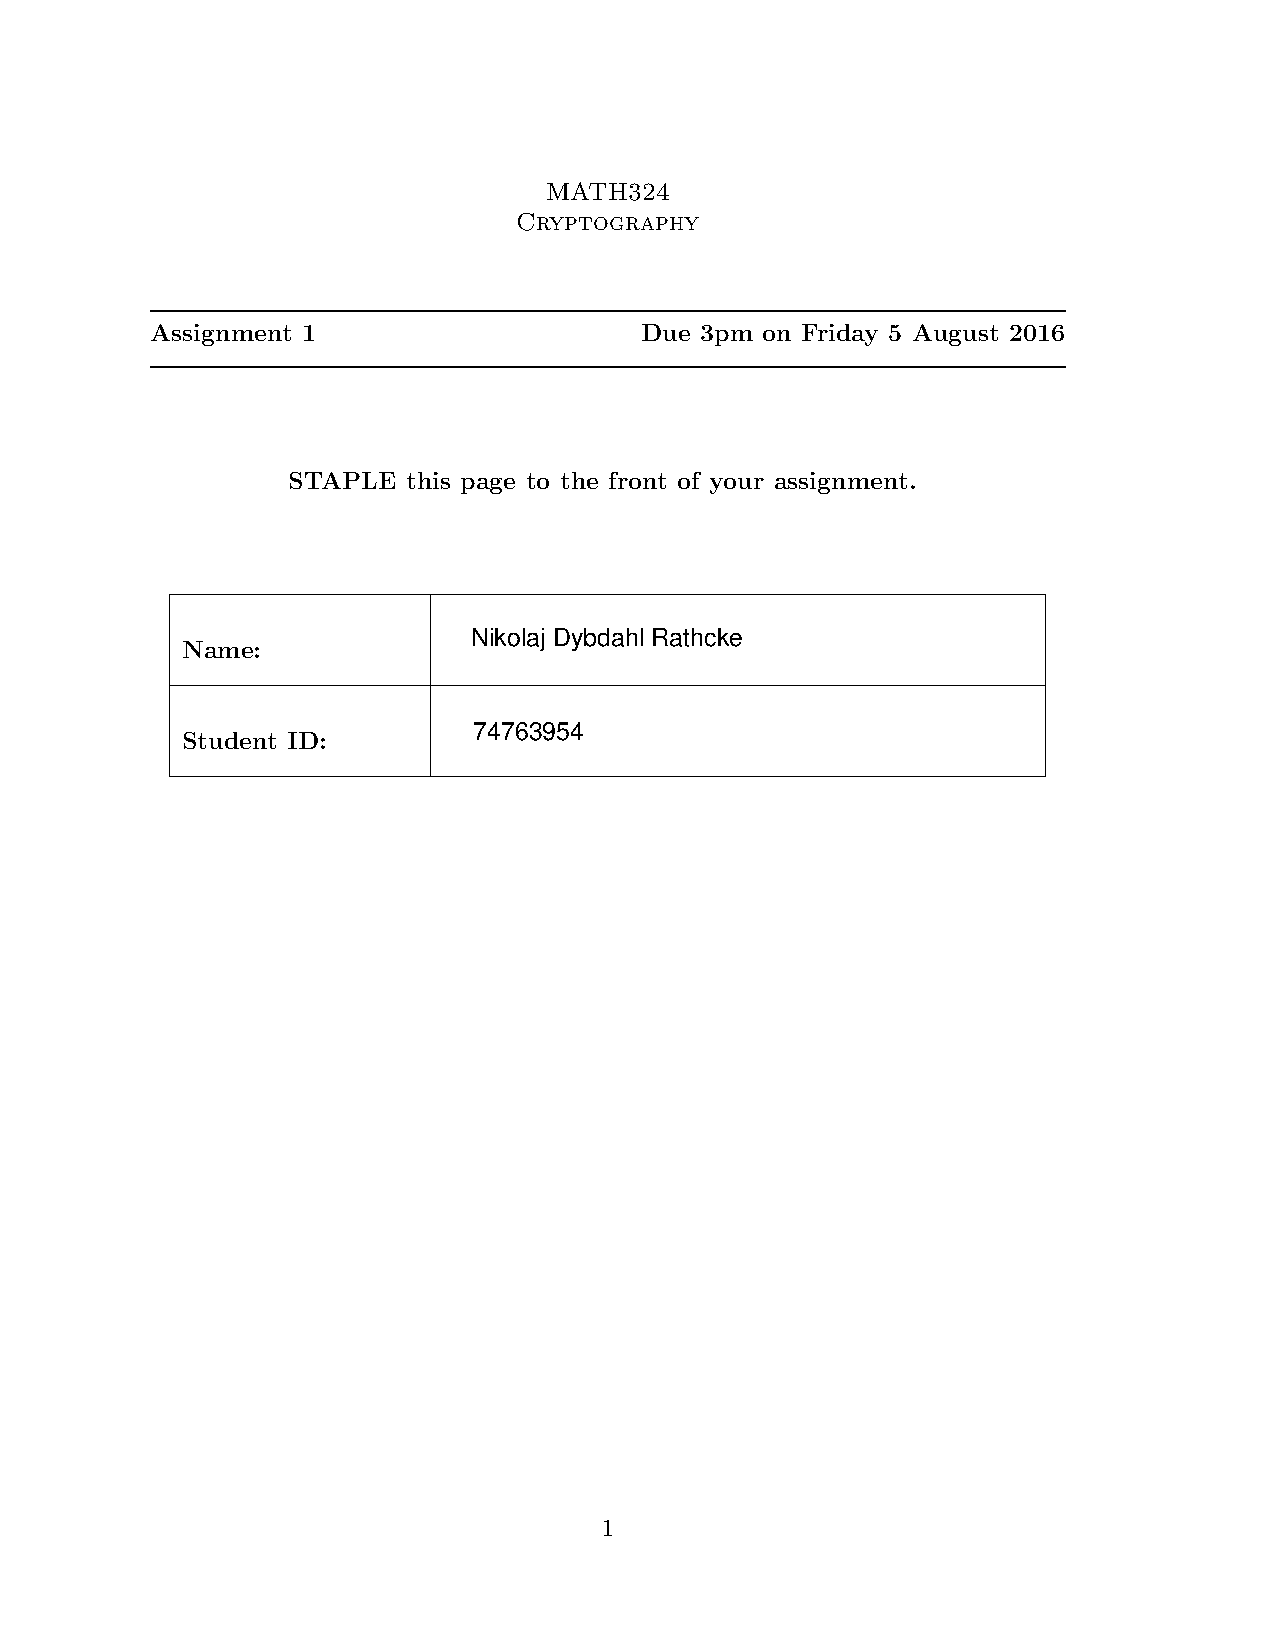
\includepdf[pages=1]{title.pdf}

\section{Question 1}
\subsection{(i)}
The key generation works by picking two large primes $p$ and $q$. We then compute $n=pq$, which is the cyclic group we are working in. We then compute $\phi(n)$ and pick some element $e$ such that $1<e<\phi(n)$ and $\gcd(e,\phi(n))=1$. The encryption key, better known as the public key, is then $(n,e)$. \\
After having picked $e$, we compute:
\begin{align}\label{eq1}
  d\equiv e^{-1} \mbox{ (mod $\phi(n)$)}
\end{align}
The decryption key, or private key, is then $(n, d)$. Note that a potential attacker does not know $p,q$ or $\phi(n)$, so $d$ is not easily computed for the attacker.

\subsection{(ii)}
The encryption function of a message $m$ is:
\begin{align*}
  c\equiv m^e \mbox{ (mod $n$)}
\end{align*}
where $0\leq m\leq n$ and $\gcd(m,n)=1$. This produces the ciphertext $c$. To decrypt this message, we compute
\begin{align*}
  m \equiv c^d \mbox{ (mod $n$)}
\end{align*}
These are inverse functions because:
\begin{align*}
  m \equiv c^d \equiv (m^e)^d \equiv m^{ed} \mbox{ (mod $n$)}
\end{align*}
Now, we have picked $d$, such that $ed\equiv 1$ (mod $\phi(n)$), so we have
\begin{align*}
  m^{ed}\equiv m^1\equiv m \mbox{ (mod $n$)}
\end{align*}
For encryption function $f(x)$ and decryption function $g(x)$, this proof applies both ways as \begin{align*}
  (m^e)^d\equiv (m^d)^e\equiv m^{ed} \mbox { (mod $n$)}
\end{align*}
This means we have:
\begin{align*}
  f(g(x))=g(f(x))=x
\end{align*}
which completes the proof.

\subsection{(iii)}
If integer factorization was easy, an attacker would be able to find the primes $p$ and $q$ from $n$. Using this, the attacker knows $\phi(n)$, since $\phi(n)=\phi(p)\phi(q)=(p-1)(q-1)$, and he could then find $d$ in Equation \ref{eq1}. Since the attacker knows $d$, he can decrypt any message $m$.

\section{Question 2}
\subsection{(i)}
The choice $e=4445$ is a bad choice as it is not invertible $\mathbb{Z}_{\phi(n)}$ where $\phi(n)=11200$, so we do not have a decryption key.

\subsection{(ii)}
With $e=3533$, the decryption key $d$ is $6597$, as $6597\equiv 3533^{-1}$ (mod $11200$).

\section{Question 3}
\subsection{(i)}
Given two public keys $(n_1, e_1)$ and $(n_2, e_2$, where $n_1$ and $n_2$ share a common prime factor, we are able to find it by simply calculating $\gcd(n_1, n_2)$ since it a factor in both numbers. This is not hard to compute if we use an algorithm such as Euclids Algorithm. From this, we can now easily find the other prime factors in the two numbers as it is only one unknown.

\subsection{(ii)}
So we calculate $\gcd(12091, 32849)$ with Euclids algorithm:
\begin{align*}
  32849 &= 2\cdot 12091 + 8667 \\
  12091 &= 1\cdot 8667  + 3424 \\
  8667  &= 2\cdot 3424  + 1819 \\
  3424  &= 1\cdot 1819  + 1605 \\
  1819  &= 1\cdot 1605  + 214  \\
  1605  &= 7\cdot 214   + 107  \\
  214   &= 2\cdot 107   + 0
\end{align*}
So the two numbers share the divisor $p=107$. We can then find the other prime factor, $q$, of $n_1=12091$:
\begin{align*}
  q &= 12091 / 107 \\
    &= 113
\end{align*}
And the prime factor, $r$, of $n_2=32849$:
\begin{align*}
  r &= 32849 / 107 \\
    &= 307
\end{align*}
And from this, we can also compute the two private keys.

\section{Question 4}
\subsection{(i)}
The idea behind the algorithm is that given an integer $n$ with prime factorization $pq$ (in RSA) and another integer $M$, where we know $p-1| M$, we know that there must exist some $k$ that satisfies $M=k(p-1)$. \\
Now, say we compute $a^M-1$ for some $a$, then if $a$ is coprime to $p$, we have that:
\begin{align*}
  a^M &\equiv a^{k(p-1)} \\
      &\equiv (a^{p-1})^k \\
      &\equiv 1^k \comment {By Fermat's little theorem} \\
      &\equiv 1 \mbox{ (mod $p$)}
\end{align*}
This means that $p|a^M-1$, so $\gcd(a^M-1, n)$ is either $p$ or $n$, so we would know if we found a prime factor. \\
There are different ways to pick $M$, but one way is to pick let it be factorials $\{1!, 2!, 3!, \ldots\}$ as they have a lot of divisors. This means that this algorithm can be explained as follows:
\begin{algorithm}[H]
  \caption{Pollard's $p-1$ algorithm}\label{alg1}
  \begin{algorithmic}[1]
    \Require{An integer $n$}
    \Statex
      \State Pick an $a$, such that $1<a<n$
      \For{$i \gets 1, 2, \ldots$}
      \State $r=\gcd(a^{i!}-1, n)$
      \If{$r=n$}
        \State Restart algorithm with new $a$
      \EndIf
      \If{$r=1$}
        \State Increment $i$, continue loop
      \EndIf
      \If{$r>1$}
        \State Then we found a prime factor in $r$, so break out of loop
      \EndIf
      \EndFor
      \State \Return $r$
  \end{algorithmic}
\end{algorithm}
Now, that we have found a prime factor, we are able to factorize $n$ in the RSA cryptosystem. Note that $a^i$ easily becomes huge, but since we are calculating the greatest common divisor, we only need to calculate $a^i-1$ modulo $n$, which is easier to compute.

\subsection{(ii)}
We can make it more resistant to these kinds of attack by ensuring that $p-1$ and $q-1$ contains one large prime factor, since Pollard's $p-1$ algorithm relies on one of the primes having the composite number $p-1$ to be a product of small primes.

\subsection{(iii)}
We start by picking $a=2$. Then with $n=713$, we follow Algorithm \ref{alg1}:
\begin{align*}
  r &= \gcd(2^{1!}-1, 713) &= &\ 1 \comment{Increment $i$} \\
  r &= \gcd(2^{2!}-1, 713) &= &\ 1 \comment{Increment $i$} \\
  r &= \gcd(2^{3!}-1, 713) &= &\ 1 \comment{Increment $i$} \\
  r &= \gcd(2^{4!}-1, 713) &= &\ 1 \comment{Increment $i$} \\
  r &= \gcd(2^{5!}-1, 713) &= &\ 31\comment{Found a prime factor!}
\end{align*}
The algorithm terminates and we found a prime factor $p=31$. We can the easily find the other prime factor $q$:
\begin{align*}
  q &= 713/31 \\
    &= 23
\end{align*}
So we have $713=31\cdot 23$!

\end{document}
